\documentclass{article}
\usepackage[utf8]{inputenc}
\usepackage{geometry}
\usepackage[colorlinks=true,linkcolor=blue,citecolor=blue,urlcolor=blue]{hyperref}
\usepackage{apacite}
\usepackage{graphicx}
\usepackage{amsmath}
\usepackage{appendix} 

\geometry{a4paper, margin=1in}
\bibliographystyle{apacite}

\newcommand{\COtwo}{CO$_2$}
\newcommand{\CHfour}{\ensuremath{\mathrm{CH}_4}}
\newcommand{\NOtwo}{\ensuremath{\mathrm{NO}_2}}
\newcommand{\McubeS}{\ensuremath{\mathrm{m}_3/s}}
\newcommand{\SOtwo}{\ensuremath{\mathrm{SO}_2}}
\newcommand{\NOx}{\ensuremath{\mathrm{NO}_x}}
\newcommand{\SOx}{\ensuremath{\mathrm{SO}_x}}
\newcommand{\PMtwoFive}{\ensuremath{\mathrm{PM}_{2.5}}}
\newcommand{\gs}{\ensuremath{\mathrm{g/s}}}
\newcommand{\Hr}{\ensuremath{H_{\mathrm{r}}}}
\newcommand{\DeltaHc}{\ensuremath{\Delta H_{c}}}
\newcommand{\GramMeterCube}{\ensuremath{\mathrm{g/m}^3}}

\newcommand{\heatReleaseRate}{
    H_{r} = \dot{m} \cdot \Delta H_{c}
}

\title{\textbf{Meteorological Influence on Gas Flaring Emissions Dispersion from the Hibernia Platform in Newfoundland and Labrador.}}
\author{Shedrach Ezenwali}
\date{\today}

\begin{document}
\maketitle

\section{Introduction}
Gas flaring emissions from offshore oil and gas platforms can pose significant environmental and health risks due to the release of pollutants. Studies have demonstrated that flaring can result in elevated levels of \NOx\ and \SOtwo, which act as precursors to acid rain and ground-level ozone formation, impacting both local and regional air quality \cite{fawole2019dispersion}. Moreover, particulate matter (\(\PMtwoFive\)) from flaring activities can contribute to respiratory and cardiovascular ailments \cite{khaleghi2023methane}. Therefore, effective monitoring and regulation are essential to mitigate these impacts.

In the assessment of dispersion and concentration, meteorological conditions such as wind speed, temperature, and humidity are crucial factors. High wind speeds are advantageous as they aid in dispersing pollutants, thus reducing their concentrations at ground level. Conversely, low wind speeds can lead to higher pollutant concentrations near the source. Temperature inversions exacerbate air quality issues by trapping pollutants close to the ground within a layer of warm air \cite{an2016atmospheric}. Moreover, the physical attributes of the flare, including its height and heat content, significantly influence dispersion patterns. Taller flares generally disperse pollutants over a wider area, while shorter flares with lower heat content can cause higher concentrations of pollutants near the emission source \cite{mirrezaei2019impact}.

Considering the stochastic nature of pollutant dispersion, variables such as the distance from source, meteorological conditions, and topography should be taken into account when selecting statistical sample points, which can be a costly endeavor. Consequently, simulation is essential to cover a range of potential scenarios \cite{fawole2019dispersion,christoudias2014atmospheric}.

\subsection{Study area}
The Hibernia platform, one of the largest offshore oil production facilities in Newfoundland and Labrador, Canada and positioned at latitude $46.75^\circ$ and longitude $-48.78^\circ$, is a significant source of gas flaring emissions. The platform's remote offshore location presents distinct challenges for monitoring and managing these emissions, In line with these considerations, this study seeks to examine how meteorological conditions influence the dispersion of gas flaring emissions from the Hibernia platform using the AERMOD dispersion model. This work concentrate on key pollutants such as \SOtwo, \NOx, and \PMtwoFive, exploring how factors like wind speed, temperature, and humidity impact their dispersion patterns. By simulating various meteorological scenarios, the research aims to shed light on potential impacts on air quality in nearby coastal regions and to provide insights into strategies for mitigating adverse effects.

The subsequent sections outline a systematized review, research methodology, including input data, validation plan, and model boundaries.

% Literature Review


\section{Literature Review}
Given the significant health and environmental consequences associated with flaring, a diverse array of modeling techniques has been employed to assess and mitigate these impacts. A systematized review of the literature underscores the importance of such methods, yet highlights a critical research gap: the need for studies that specifically address the influence of meteorological conditions on gas flaring emissions and their dispersion patterns, particularly in unique geographical locales like the Hibernia Platform in Newfoundland and Labrador.

Recent research offers various approaches to understanding pollutant dispersion from flaring. \cite{popovicheva2022siberian} applied a Lagrangian particle dispersion model to assess how emissions in Arctic flaring sites are affected by cold weather conditions and low-level inversions, suggesting a complex interaction between weather conditions and pollutant behavior. Similarly, \cite{miao2014multi} utilized a multi-layer atmospheric model to explore the vertical and horizontal spread of emissions in urban environments. Additionally, \cite{caseiro2023quantification} integrated satellite observations with ground-based sensors to track and quantify flaring emissions in Persian Gulf between Qatar and Iran, providing a comprehensive framework to understand dispersion patterns over time, an approach that could be adapted to the isolated settings of Newfoundland and Labrador.

To further emphasize the impact of weather on dispersion, a study by \cite{fawole2019dispersion,nwosisi2020dispersion} investigated how varying wind speeds and directions affect the dispersion of pollutants in coastal areas, revealing significant variability in dispersion patterns based on wind conditions alone. Another pertinent study by \cite{henao2017direct} analyzed the effect of precipitation on the deposition and dispersion of particulate matter, showing that wet conditions can substantially alter the fate of airborne pollutants. Additionally, \cite{wallace2010topographic} explored the impact of temperature inversions on air quality, demonstrating how such meteorological phenomena can trap pollutants close to the ground, exacerbating local air quality issues.

These insights into the meteorological influences on dispersion provide a crucial backdrop for the introduction of AERMOD. Central to our discussion, AERMOD is a sophisticated atmospheric dispersion model developed by the U.S. Environmental Protection Agency (EPA). It is designed to estimate pollutant concentrations by incorporating both emissions data and meteorological influences, making it ideal for regulatory and environmental impact assessments. Studies by \cite{cimorelli2005aermod,amoatey2019performance} have highlighted AERMOD's effectiveness in modelling complex dispersion patterns across various terrains and handling emissions from multiple sources, respectively.

Further leveraging AERMOD, \cite{afzali2017prediction} also validated AERMOD's precision in modelling pollutant dispersion over coastal regions affected by land-sea breezes, crucial for areas like Newfoundland and Labrador.

Considering the robustness and adaptability of AERMOD, it has been selected for our study on the Hibernia Platform. This model's integration of complex meteorological data and varied emission scenarios will be invaluable in accurately predicting the dispersion of flaring emissions under the distinctive environmental conditions of Newfoundland and Labrador. This approach aims to provide a detailed assessment of potential air quality impacts and contribute to more effective environmental management practices in the region.
\section{Methodology}
This section provides an in-depth description of the modeling setup, the emission rates from flaring activities at the facility, the meteorological parameters employed, and the composition of the gas burnt which are input data for the AERMOD model as illustrated in figure \ref{data-input-aermod}
\subsection{Meteorological Data}

In AERMOD dispersion modeling, precise meteorological data plays a pivotal role. Both surface and upper air data are typically essential for capturing the atmospheric conditions that impact pollutant dispersion. However, due to the unavailability of upper air sounding data, this study exclusively utilizes surface meteorological data. This includes hourly measurements of temperature, wind direction and speed, relative humidity, and station pressure. Throughout the model year, prevailing wind directions were observed to be west during winter and west-southwest in summer. Temperature fluctuations ranged from -11°C to 25°C.

To address the absence of upper air sounding data, AERMOD employs a methodology that estimates the required upper air parameters based on available surface data. This method involves using default vertical profiles or adjusting them based on surface data to approximate the effects of atmospheric stratification and mixing heights on pollutant dispersion. This ensures robust modeling and an accurate representation of dynamic atmospheric conditions.

\subsection{Stack Physical Parameters:}
The stack on the platform has a height of 47 meters and a diameter of 3 meters, as specified in a previous modelling of the Hebron Project \cite{Hebron2010}.

\subsection{Emission and Combustion Parameters in Dispersion Modeling}

For this study, we simulated the dispersion of \NOtwo, CO, and \PMtwoFive. The emission rates from this facility, averaged for 2022, are 30 \gs, 38.5 \gs, and 3.7 \gs~respectively. The gas volume flared from this facility is estimated using satellite sensors, and for our case, it is 41 m\textsuperscript{3}/s in 2022 \cite{WorldBankFlaring}.

To model the dispersion of emissions from flaring accurately, pseudo-parameters such as effective stack height, effective exit velocity, and effective stack diameter are calculated. These parameters simulate the plume's behavior as if emitted from a point source at the flame tip, accounting for air entrainment, buoyancy, heat loss due to radiation (assumed  25\% as suggested by \cite{idriss2003emergency}) and momentum. This approach ensures more accurate plume rise and dispersion predictions in advanced models like AERMOD, preventing underestimation of pollutant concentrations at ground level \cite{Ontario2024}.

The mass flow rate $\dot{m}$ was calculated from the volume flow rate using a gas density range of 600 to 900 \GramMeterCube, as recommended by \cite{elsharkawy2004efficient}. Flared gas consists of various components, with methane being the primary compound by mole fraction. The detailed composition utilized in this study can be found in Table~\ref{tab:gas_composition}.

\noindent 1. \text{Heat Release Rate}: $H_r$, 2. \text{Enthalpy Change}: $\Delta H_c$, 3. \text{Buoyancy Flux}: $F_b$, 4. \text{Momentum Flux}: $F_m$, 5. \text{Exit Gas Temperature}: $T_{exit}$, 6. \text{Effective Stack Height}: $H_{eff}$, 7. \text{Effective Stack Diameter}: $D_{eff}$, 8. \text{Effective Exit Velocity}: $V_{eff}$.


\begin{equation}
    \label{eq:heatRelease}
    H_{r} = \dot{m} \cdot \DeltaHc \cdot F_{r}
\end{equation}

\begin{equation}
    \label{eq:enthalpyChange}
    \DeltaHc = \sum (x_{i} \cdot \Delta H_{c,i})
\end{equation}



\begin{table}[h]
    \centering
    \caption{Gas composition parameters} 
    \label{tab:gas_composition}
    \begin{tabular}{|c|c|c|c|}
    \hline
    Compound & Formula & Percent in Natural Gas & \(\Delta H_c \) (KJ/g) \\ \hline
    Methane & CH\(_4\) & 96.6428 & -55.5 \\ \hline
    Ethane & C\(_2\)H\(_6\) & 0.8981 & -51.9 \\ \hline
    Propane & C\(_3\)H\(_8\) & 0.1095 & -50.3 \\ \hline
    Butane & C\(_4\)H\(_{10}\) & 0.04 & -49.5 \\ \hline
    Carbon Dioxide & CO\(_2\) & 0.5021 & -8.94 \\ \hline
    \end{tabular}
\end{table}



\begin{equation}
    F_b = g \times \frac{H_r}{\pi \times \rho_{\text{air}} \times T_{\text{ambient}} \times C_p} 
\end{equation}

\begin{equation}
    F_m = \frac{V_s H_r}{\pi C_p \rho_a (T_{exit} - T_{ambient})} 
\end{equation}



\begin{equation}
T_{exit} = T_{ambient} + \frac{H_r}{\dot{m} \cdot C_p}
\end{equation}


\begin{equation}
    H_{\text{eff}} = H_{\text{actual}} + (4.56 \times 10^{-3} \times \left( \frac{H_r}{4.1868} \right)^{0.478} 
\end{equation}

\begin{equation}
    D_{\text{eff}} = 2 \times \sqrt{\frac{(F_b \times T_{\text{exit}})}{g \times V_{\text{eff}} \times (T_{\text{exit}} - T_{\text{ambient}})}} 
\end{equation}

\begin{equation}
    V_{\text{eff}} = g \times \frac{F_m}{F_b} \times \frac{(T_{\text{exit}} - T_{\text{ambient}})}{T_{\text{ambient}}} 
\end{equation}



Where:
\begin{itemize}
    \item $\dot{m}$: Mass flow rate of the gas (g/s)
    \item $F_r$: Heat loss fraction due to radiation
    \item $C_p$: Specific Heat Capacity of air (J/g·K)
    \item $T_{ambient}$: Ambient temperature (K)
    \item $x_i$: Mole fraction of each gas component
    \item $\Delta H_{c,i}$: Heat combustion enthalpy for each gas component (J/g)
    \item $H_r$: Heat release rate (J/s)
    \item $\rho_{\text{air}}$: Density of air (g/m³)
    \item $V_s$: Acutal velocity (m/s)
    \item $H_{\text{actual}}$: Actual flare height (m)
    \item $g$: Acceleration due to gravity (m/s²)
    \item $\rho_a$: Density of air at specific conditions (g/m³)
\end{itemize}


\subsection{Terrain Data}
This an offshore platform there is no need for a terrain data, as the surrounding area is predominantly water without significant elevation changes.

\subsection{Model Boundaries and Domain}
The model boundaries and domain are defined as follows:

\noindent \textbf{Horizontal Boundaries:} The horizontal boundaries extend 5 km in all directions from the Hibernia platform. 


\noindent \textbf{Spatial Resolution:} A grid resolution of 1 km x 1 km is utilized across the modeling domain, with finer resolutions of 500 m x 500 m applied near the platform to capture detailed variations in pollutant concentrations.

\noindent \textbf{Temporal Resolution:} Hourly meteorological data is employed to capture the temporal variations in atmospheric conditions. The simulation covers a full year to account for seasonal variations in emissions and meteorological conditions.

\noindent \textbf{Key Consideration:} The flare stack on the platform is accurately represented within the domain, all other emission sources are excluded.

\section*{Model Result Validation Plan}
The purpose of this validation plan is to verify the accuracy and dependability of the AERMOD dispersion model results for the Hibernia platform. This will be achieved by comparing the results with a  air emissions and dispersion modeling report conducted for the Hebron Project by Stantec Consulting Ltd. in June 2010 \cite{Hebron2010}. It is important to note that the Hebron Project report has some limitations, such as the use of pseudo-parameters and an unclear model domain in relation to emissions from other sources. These limitations will be carefully considered during the validation process.

\section*{Validation Steps}

\begin{enumerate}
    \item \textbf{Data Comparison}:
    \begin{itemize}
        \item Once the AERMOD simulation is completed, we  will extract pertinent data from the Hebron Project report, such as emission rates, stack parameters, and dispersion modeling results for similar pollutants.
        \item Address the limitations identified in the Hebron Project report by adjusting for pseudo-parameters and ensuring that only comparable emission sources are taken into account.
    \end{itemize}
    
    \item \textbf{RMSE Calculation}:
    \begin{itemize}
        \item Calculate the Root Mean Square Error (RMSE) to quantify the differences between this predictions and Hebron Project results.
        \[
        \text{RMSE} = \sqrt{\frac{1}{n} \sum_{i=1}^{n} (P_{\text{AERMOD},i} - P_{\text{Hebron},i})^2}
        \]
        where \( P_{\text{AERMOD},i} \) is the predicted value by AERMOD model, \( P_{\text{Hebron},i} \) is the value from the Hebron Project report for \(i \in \{\text{CO}, \text{NO}_2, \text{PM}_{2.5}\}\), and \( n \) is the number of observations.
    \end{itemize}
\end{enumerate}
By comparing AERMOD predictions with the Hebron Project study, this validation plan aims to ensure the model's accuracy, considering the identified limitations. 


\begin{figure}[h]
    \centering
    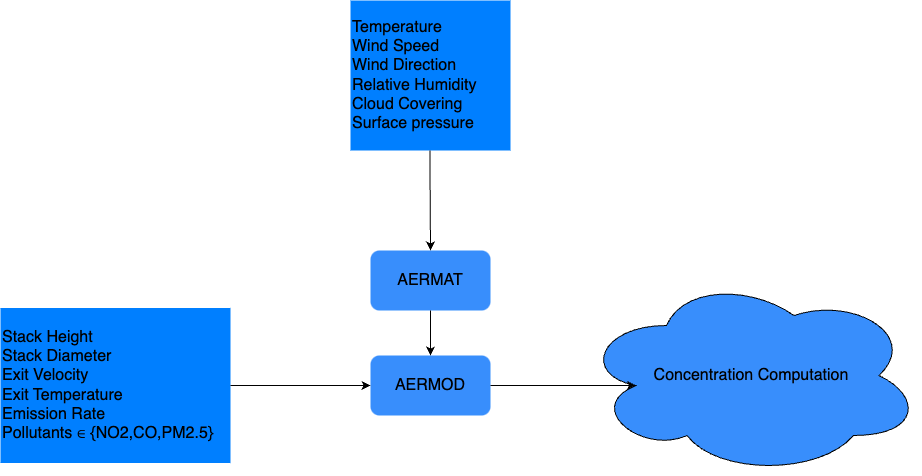
\includegraphics[width=0.8\textwidth]{./assets/flow_chart.png}
    \caption{Data input for AERMOD.}
    \label{data-input-aermod}
\end{figure}
    
% \section*{Keywords}
\begin{itemize}
    \item Gas flaring emissions
    \item Dispersion modeling
    \item Meteorological conditions
    \item Oil and Gas
    \item Aermod
\end{itemize}

\section*{Search Streams, Database, No. of Hits}
\begin{enumerate}
    \item Gas flaring emissions dispersion modelling, Google Scholar, 20,000 hits
    \item Newfoundland and Labrador gas flaring dispersion AND meteorological conditions, Google Scholar, 783 hits
    \item Impact of weather on gas flaring emissions dispersion, Google Scholar, 17,700 hits
    \item Gas flaring dispersion patterns and meteorological conditions, Google Scholar, 17,800 hits
\end{enumerate}
\section*{Inclusion/Exclusion Criteria}
\begin{itemize}
    \item Newer than 2016
    \item With exact phrase oil and gas
    \item Contains Aermod
\end{itemize}

\section*{Search Streams, Filtered Literature and Nos. of Papers}
\begin{enumerate}
    \item Search stream 1, applied inclusion/exclusion criteria, reduced to 111 papers
    \item Search stream 2, applied inclusion/exclusion criteria, reduced to 5 papers
    \item Search stream 3, applied inclusion/exclusion criteria, reduced to 108 papers 
    \item Search stream 5, applied inclusion/exclusion criteria, reduced to 80 papers
\end{enumerate}

\section*{Synopsis}

\subsection*{Paper 1}
\textbf{Title:} Dispersion of gas flaring emissions in the Niger delta: Impact of prevailing meteorological conditions and flare characteristics \cite{fawole2019dispersion}.\\
\textbf{Summary:} This study investigates the relationship between meteorological conditions, flare characteristics (such as size), and their impact on the dispersion and ground-level concentrations of pollutants from gas flares in the Niger Delta. The research aims to address a significant gap in understanding the real-world effects of gas flares on air quality, through extensive data gathered from flaring activities in the oil and gas industry. Using ADMS 5 and AERMOD dispersion models, the researchers simulated pollutant dispersion under various conditions. Findings indicate that during the West African Monsoon (WAM) months (April to September), pollutants primarily disperse over inland communities, while during non-WAM months (November to March), they disperse towards both inland and coastal areas. Smaller flares and those with lower heat content resulted in higher pollutant concentrations near the flares. The study suggests mitigating local pollution by combining short stacks flaring at lower volumes to enhance plume buoyancy, reducing ground-level concentrations. This research shows the significant impact of flare characteristics and meteorology on pollution dispersion and the necessity for strategic measures to enhance air quality.
\subsection*{Paper 2}
\textbf{Title:} Methane emission rate estimate using airborne measurement at offshore oil platforms in Newfoundland and Labrador, Canada \cite{khaleghi2023methane}.\\
\textbf{Summary:} The study addresses the knowledge gap in methane (\(\CHfour\)) emissions from offshore oil production in Newfoundland and Labrador, which previously lacked targeted measurements despite low emission intensities reported by the industry. The researchers used a Twin Otter aircraft equipped with a Picarro gas analyzer and an Aventech wind system to measure \CHfour\ emissions from three offshore oil facilities. They applied two methods: the Top-down Emission Rate Retrieval Algorithm (TERRA) and the Gaussian Dispersion method (GD). Key findings reveal that emission rates ranged from 2,890 to 7,975 m3 \CHfour\ per day, aligning closely with federal estimates. The calculated methane intensities suggest that Canadian offshore production has lower methane intensity compared to onshore production, implying more efficient and potentially safer production practices. This research highlights the importance of accurate emissions measurement to inform regulation and mitigation strategies for offshore oil production.


\subsection*{Paper 3}
\textbf{Title:} Evaluating CO, \NOtwo\, and \SOtwo\ Emissions From Stacks of Turbines and Gas Furnaces of Oil and Gas Processing Complex Using AERMOD \cite{mousavi2022evaluating}.\\
\textbf{Summary:} The research delves into the issue of air pollution originating from industrial sources, specifically the emissions from the stack of turbines and gas furnaces at Maroon oil and gas facilities in Iran. The study aims to fill the knowledge gap in accurately modeling pollutant dispersion using the AERMOD model. After calculating the emission rates, the dispersion was simulated over a 2500 km² area, and the results were verified through field measurements. The study found that pollutant concentrations were higher during the cold season but remained within the limits set by Iranian and US EPA standards. These findings highlight the effectiveness of AERMOD in predicting pollutant dispersion and stress the importance of continuous monitoring and potential mitigation measures, such as the installation of filters and electric compressors, to further reduce emissions and protect public health.


\subsection*{Paper 4}
\textbf{Title:} Dispersion and emission patterns of \NOtwo\ from gas flaring stations in the Niger Delta, Nigeria \cite{nwosisi2020dispersion}.\\
\textbf{Summary:} The research addresses the knowledge gap related to the spatial and temporal patterns of \NOtwo\ emissions from gas flaring stations and their impact on human health and the environment. The study, conducted from January 2017 to December 2018, utilized Aeroqual gas monitors and the HYSPLIT model to measure and forecast \NOtwo\ dispersion from eight gas flaring stations. The findings revealed higher \NOtwo\ concentrations in 2017 compared to 2018, with peak levels during the rainy season. Meteorological factors such as temperature, humidity, and wind speed affected \NOtwo\ concentrations, leading to lower dispersion during low wind speeds. The study underscored the significant spread of \NOtwo\ to non-oil producing states, emphasizing the necessity for protective measures for vulnerable populations.

\subsection*{Paper 5}
\textbf{Title:} Impact of Meteorological Parameters on Dispersion Modeling of Sulfur Dioxide from Gas Flares (Case Study: Sirri Island) \cite{mirrezaei2019impact}.\\
\textbf{Summary:} The paper addresses the knowledge gap in modelling the dispersion of \SOtwo\ from gas flares in coastal areas, particularly on islands with varying meteorological and terrain parameters. The research methodology utilized the CALPUFF dispersion model, a non-steady-state Lagrangian puff model, in conjunction with the Weather Research and Forecasting (WRF) model to simulate the dispersion of \SOtwo\ from flares on Sirri Island in the Persian Gulf over two five-day periods (from
29 January 2011 to 2 February 2011 and 20 October to 24
October 2011). The study incorporated flare parameters based on EPA guidelines into the model. The key findings indicate that low-height flares have a significant impact on ground-level \SOtwo\ concentrations, whereas elevated flares affect areas farther from the flaring site. The results emphasize the importance of considering local meteorological conditions and terrain in air pollution modelling, highlighting the effectiveness of coupling the CALPUFF-WRF models in accurately predicting pollutant dispersion in complex environments.

\subsection*{Paper 6}
\textbf{Title:} Emissions Dispersion Simulated For A Crude Oil Tank Farm Explosion In The Niger Delta Of Nigeria \cite{edeemissions}.\\ 
\textbf{Summary:} This research investigates the environmental and health effects of emissions resulting from a crude oil tank explosion. One significant knowledge gap is the absence of detailed simulation studies on the dispersion of pollutants from unplanned events such as explosions, particularly considering the proximity of oil facilities to populated areas in this region. The study utilizes the AirWare Model alongside the Gaussian plume model to simulate the dispersion of emissions under varying atmospheric conditions. Emission factors, meteorological variables, and site-specific characteristics are employed to assess pollutant concentrations at different distances downwind. The study highlights that pollutants such as suspended particulate matter (SPM), nitrogen oxides (\(\NOx\)), carbon monoxide (CO), and sulphur oxides (\(\SOx\)) notably exceed both national and international air quality standards, especially under unstable atmospheric conditions. These findings emphasize the necessity for stringent regulatory measures and the use of advanced modeling techniques to effectively manage air pollution in the area.

\section*{Summary}
The significance of understanding the dispersion of pollutants from gas flaring and industrial emissions, influenced by meteorological conditions, is well emphasized in the above literature. Advanced dispersion models such as ADMS 5, AERMOD, CALPUFF, and HYSPLIT, along with empirical measurements like the offshore platforms in Newfoundland, are crucial for accurately replicating real-world conditions and forecasting pollutant behaviour.

Research indicates that meteorological factors such as wind speed, temperature, and humidity have a significant impact on the dispersion of pollutants. For instance, in the Niger Delta, pollutants disperse inland during the WAM months and towards both inland and coastal areas in non-WAM months, affecting local communities. A similar pattern was observed in the Sirri Island study, indicating the spread of these pollutants beyond flaring sites, impacting non-oil-producing regions.

Furthermore, the characteristics of pollutants, including the size and heat content of gas flares, play a crucial role. Smaller flares with lower heat content result in higher pollutant concentrations near the source, underscoring the need for mitigation strategies to improve plume buoyancy and reduce local pollution.

In conclusion, continuous monitoring, precise modelling, and targeted mitigation are essential for managing and reducing the adverse impacts of industrial emissions on air quality and public health.

\newpage
\bibliography{references}

\begin{appendix}
    \centering 
    \section*{Appendix} 
    \subsection*{Aermod Initial Setup} 
    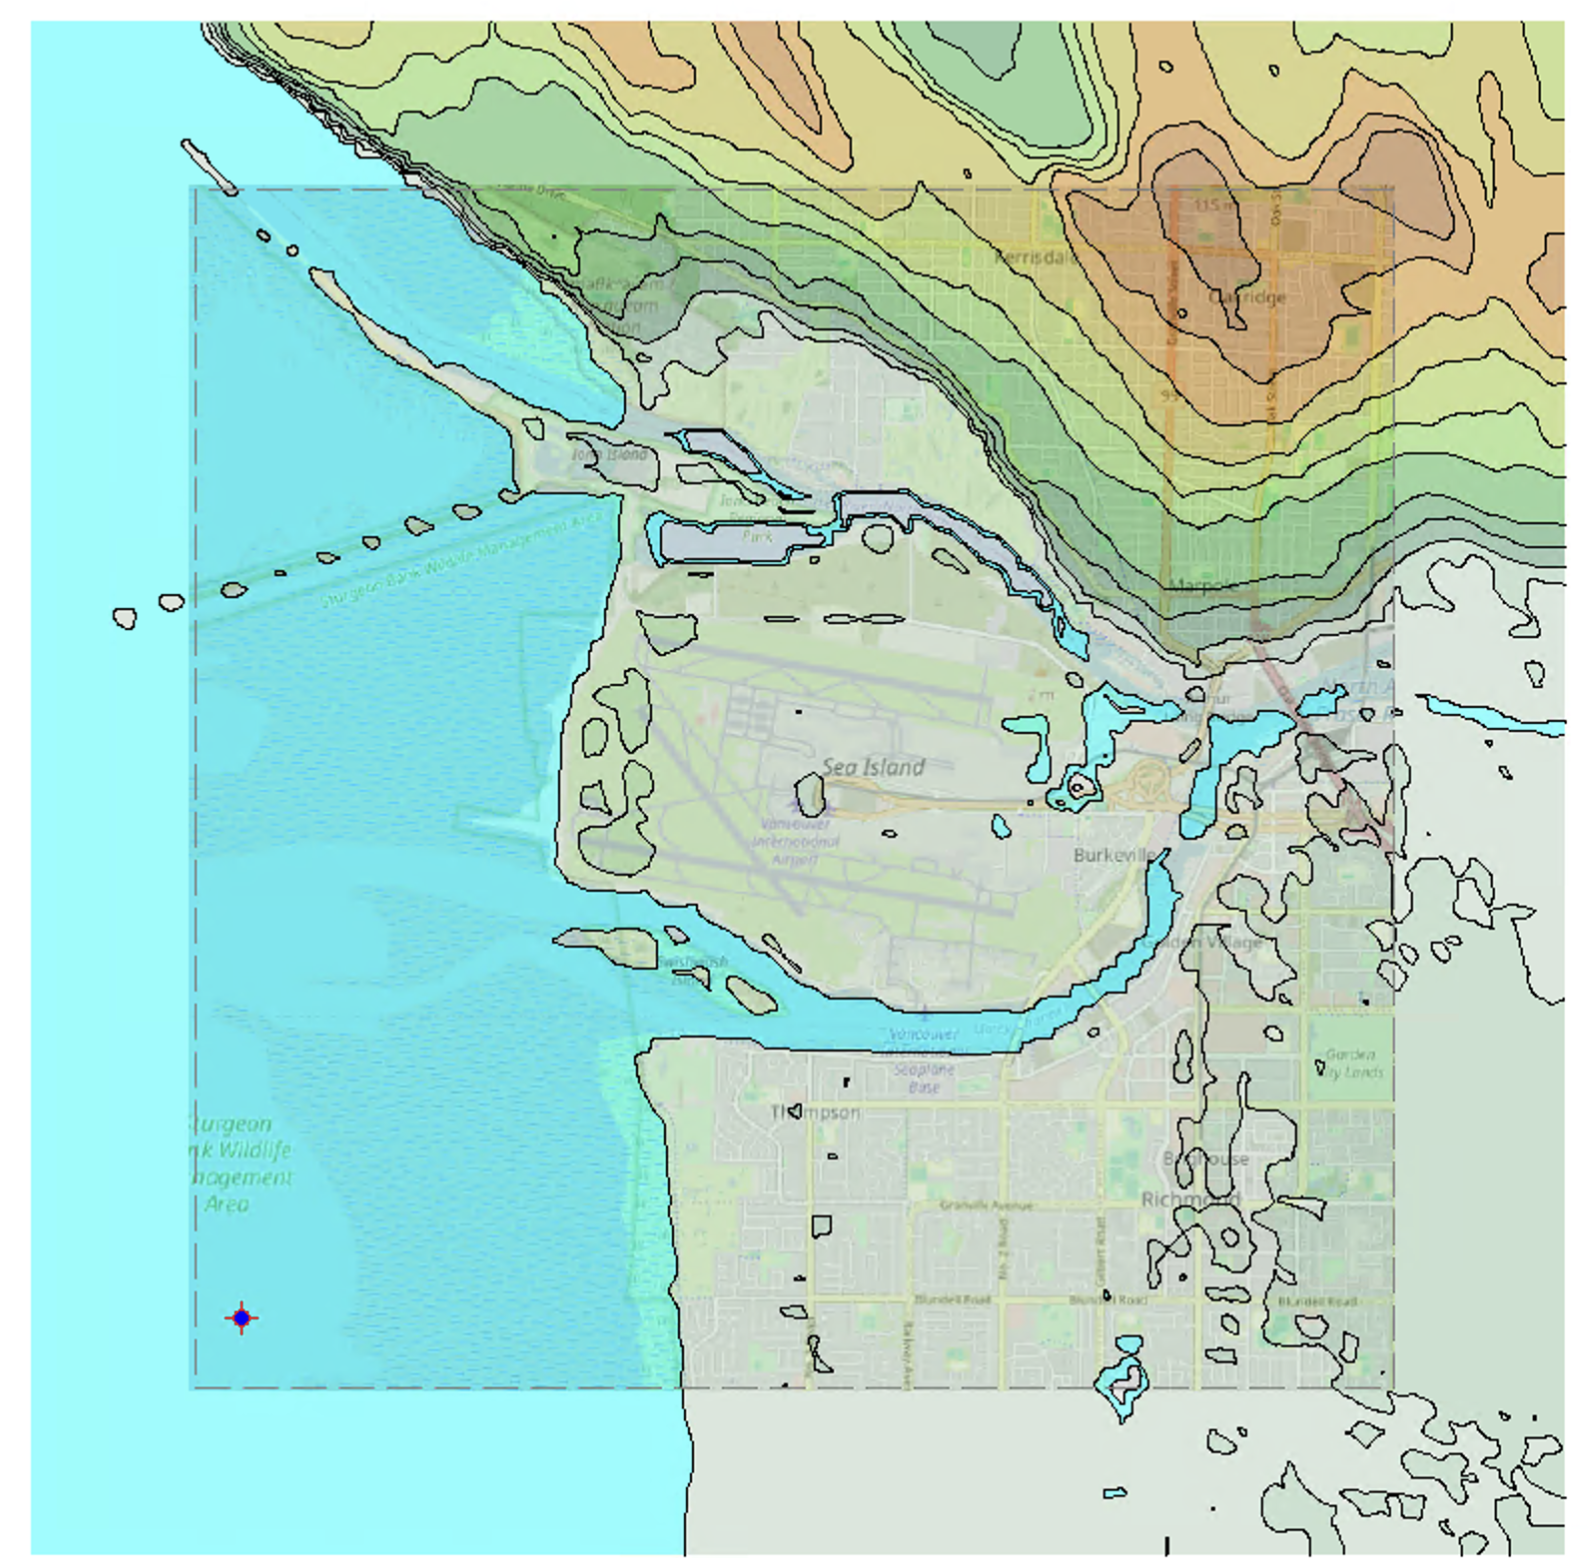
\includegraphics[width=1\textwidth]{./assets/aermod.png} 

    \subsection*{Distance from study site to closest Air monitoring station} 
    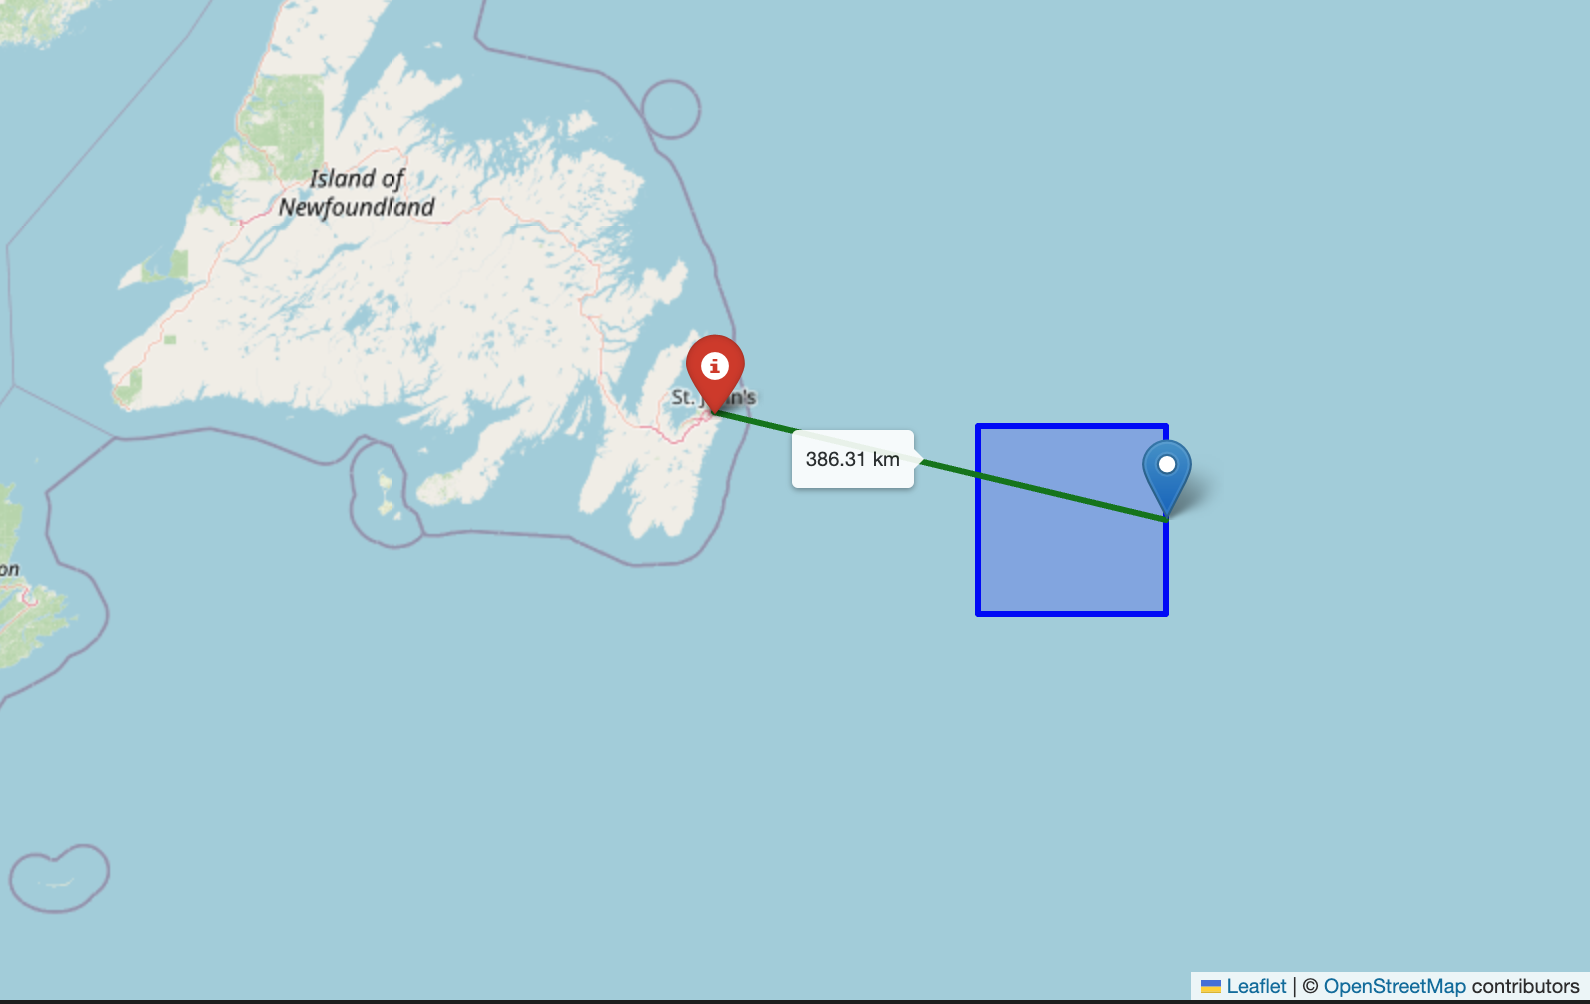
\includegraphics[width=1\textwidth]{./assets/study_site.png}
\end{appendix}
    

\end{document}
